\section{Reconnaissance de visage}
\subsection{Détection de visage}
\begin{frame}
  \frametitle{Détection de visage}
  \begin{columns}[c]
    \begin{column}[T]{.5\textwidth}
      \begin{itemize}
        \item Utilisation d'OpenCV
          \begin{itemize}
            \item open source computer vision library
          \end{itemize}
        \item Utilisation de classifieur pour la detection de visage
          \begin{itemize}
            \item Obtention d'un cercle (rayon et centre)
          \end{itemize}
      \end{itemize}
    \end{column}
    \begin{column}[T]{.5\textwidth}
      \begin{figure}
        \begin{center}
          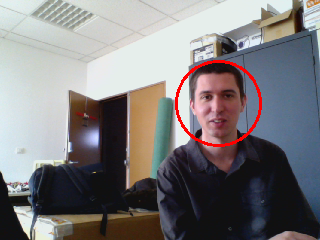
\includegraphics[width=5cm]{image/faceDetection.png}
        \end{center}
      \end{figure}
    \end{column}
  \end{columns}   
\end{frame}

\subsection{Calcul de l'ouverture}
\begin{frame}
  \frametitle{Calcul de l'ouverture}
  \begin{figure}
    \begin{columns}[c]
      \begin{column}[T]{.5\textwidth}
        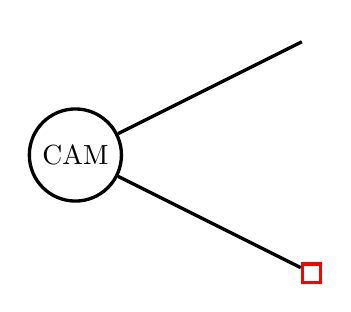
\begin{tikzpicture}[scale=0.5]
  \node[draw, circle, very thick] (CAM) at (0,3) {CAM};
  \node[draw, very thick,color=red] (TARGET) at (6,0) {};
  \node[] (NO) at (6,6) {};
  \draw[very thick] (CAM) -- (TARGET);
  \draw[very thick] (CAM) -- (NO);
\end{tikzpicture}

      \end{column}
      \begin{column}[T]{.5\textwidth}
        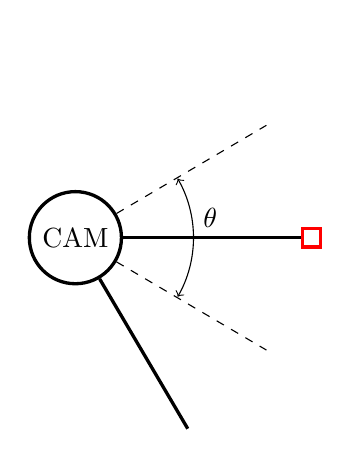
\begin{tikzpicture}[scale=0.5]
 \tikzset{directed/.style={->}} 
  \node[draw, circle, very thick] (CAM) at (0,0) {CAM};
  \node[draw, very thick,color=red] (TARGET) at (6,0) {};
  \node[] (P1) at (3,5.1) {};
  \node[] (P2) at (3,-5.1) {};
  \node[] (P3) at (5.1,3) {};
  \node[] (P4) at (5.1,-3) {};
  \draw[very thick] (CAM) -- (TARGET);
  \draw[very thick] (CAM) -- (P2);
  \draw[dashed] (CAM) -- (P3);
  \draw[dashed] (CAM) -- (P4);
  \draw[directed] (0,0) ++(3,0) node[above right] {$\theta$} arc (0:30:3cm);
  \draw[directed] (0,0) ++(3,0) arc (0:-30:3cm);
%  \fill[very thick] (0.946,0.55) circle (0.2cm);
\end{tikzpicture}


      \end{column}
    \end{columns}   
  \end{figure}
\end{frame}

\subsection{Suivi de visages}
\begin{frame}
  \frametitle{Suivi de visages}
  \begin{itemize}
    \item Déterminer :
      \begin{itemize}
        \item la distance au centre de l'image
        \item l'angle horizontal et vertical du visage par rapport au centre 
      \end{itemize}
    \item Déplacer les moteurs de la tête des angles calculés
  \end{itemize}
\end{frame}
